\documentclass[10pt]{article}

\usepackage[utf8]{inputenc}
\usepackage[T1]{fontenc}
\usepackage{lmodern}
\usepackage[a4paper,margin=0.78in]{geometry}
\usepackage{amsmath,amssymb,mathtools}
\usepackage{xcolor}
\usepackage[most]{tcolorbox}
\usepackage{booktabs,array,tabularx,longtable,multirow}
\usepackage{enumitem}
\usepackage{titlesec}
\usepackage{parskip}
\usepackage{microtype}
\usepackage{tikz}
\usetikzlibrary{arrows.meta,positioning,fit,calc}
\usepackage[colorlinks=true,linkcolor=blue!55!black,urlcolor=blue!65!black,citecolor=blue!55!black]{hyperref}
\hypersetup{
  pdftitle={Tensor, Low-Rank, and Sparse Inference Systems},
  pdfsubject={Advisor and collaborator research briefing on KV-cache compression and collaborative inference},
  pdfkeywords={KV cache, tensor decomposition, low rank, sparsity, collaborative inference}
}

\definecolor{ink}{HTML}{17223B}
\definecolor{accent}{HTML}{44318D}
\definecolor{teal}{HTML}{087F8C}
\definecolor{orange}{HTML}{C15F18}
\definecolor{green}{HTML}{287D3C}
\definecolor{red}{HTML}{A62929}
\definecolor{soft}{HTML}{F4F2FB}
\definecolor{cool}{HTML}{EAF7F8}
\definecolor{warm}{HTML}{FFF3E7}
\definecolor{graybg}{HTML}{F3F5F7}

\titleformat{\section}{\Large\bfseries\color{accent}}{\thesection}{0.55em}{}
\titleformat{\subsection}{\large\bfseries\color{accent!85!black}}{\thesubsection}{0.55em}{}
\titleformat{\subsubsection}{\normalsize\bfseries\color{teal!85!black}}{\thesubsubsection}{0.55em}{}
\titlespacing*{\section}{0pt}{1.35em}{0.45em}

\newtcolorbox{keybox}[1][]{colback=soft,colframe=accent,boxrule=.75pt,arc=2pt,
 left=7pt,right=7pt,top=5pt,bottom=5pt,fonttitle=\bfseries,#1}
\newtcolorbox{gapbox}[1][]{colback=warm,colframe=orange,boxrule=.75pt,arc=2pt,
 left=7pt,right=7pt,top=5pt,bottom=5pt,fonttitle=\bfseries,#1}
\newtcolorbox{methodbox}[1][]{colback=cool,colframe=teal,boxrule=.75pt,arc=2pt,
 left=7pt,right=7pt,top=5pt,bottom=5pt,fonttitle=\bfseries,#1}
\newtcolorbox{riskbox}[1][]{colback=red!3,colframe=red,boxrule=.75pt,arc=2pt,
 left=7pt,right=7pt,top=5pt,bottom=5pt,fonttitle=\bfseries,#1}
\newtcolorbox{statusbox}[1][]{colback=graybg,colframe=ink!55,boxrule=.65pt,arc=2pt,
 left=7pt,right=7pt,top=5pt,bottom=5pt,fonttitle=\bfseries,#1}
\newtcolorbox{donebox}[1][]{colback=green!4,colframe=green!75!black,boxrule=.7pt,arc=2pt,
 left=7pt,right=7pt,top=5pt,bottom=5pt,fonttitle=\bfseries,#1}

\newcommand{\R}{\mathbb{R}}
\newcommand{\E}{\mathbb{E}}
\newcommand{\norm}[1]{\left\lVert #1\right\rVert}
\newcommand{\Attn}{\operatorname{Attn}}
\newcommand{\softmax}{\operatorname{softmax}}
\newcommand{\bytes}{\operatorname{Bytes}}
\newcommand{\term}[1]{\textbf{\color{accent!85!black}#1}}
\newcommand{\pub}{\textcolor{green!80!black}{\textbf{P}}}
\newcommand{\pre}{\textcolor{orange!90!black}{\textbf{A}}}
\newcommand{\unpub}{\textcolor{red!85!black}{\textbf{U}}}
\newcolumntype{P}[1]{>{\raggedright\arraybackslash}p{#1}}
\newcolumntype{Y}{>{\raggedright\arraybackslash}X}

\begin{document}
\pagenumbering{roman}

\begin{titlepage}
\centering
\vspace*{0.8cm}
{\Huge\bfseries\color{accent} Tensor, Low-Rank, and Sparse\\[3pt]Inference Systems\par}
\vspace{0.35cm}
{\Large\bfseries Literature synthesis, completed design work, and proposed research portfolio\par}
\vspace{0.6cm}
\large Research briefing for advisor and collaborators\\[2pt]
Evidence cutoff: 23 July 2026\par
\vspace{0.8cm}
\begin{tcolorbox}[colback=soft,colframe=accent,width=.94\textwidth,arc=3pt]
\small
\textbf{Current recommendation.} The field has moved beyond simple KV cache compression. Strong work
now co-designs the representation, RoPE treatment, rank allocation, residual protection, and the
attention kernel. Our recommended first implementation is \textbf{SAGE-CP-KV}: a
Softmax-Aware CP tensor representation for the compressible bulk, plus attention-influence-selected
RoPE-pair sparse corrections, consumed directly without reconstructing old keys or values.
\end{tcolorbox}
\vspace{0.55cm}
\begin{tcolorbox}[colback=warm,colframe=orange,width=.94\textwidth,arc=3pt]
\small
\textbf{Novelty warning.} ``Low rank + sparsity'' is not itself a novel claim. GEAR already uses
low-rank and sparse corrections to quantization error; OjaKV keeps exact anchors around a low-rank
cache; SALS and ShadowKV use low-rank structure for sparse access; JoLT pairs Tucker factors with a
low-bit residual. A publishable paper must make the \emph{objective, sparse structure, tensor
execution, or runtime policy} genuinely different and demonstrate a new quality--memory--latency
Pareto point.
\end{tcolorbox}
\vfill
{\normalsize Advisor/collaborator research brief \;\textbullet\; editable research plan\par}
\end{titlepage}

\setcounter{page}{2}
\tableofcontents
\newpage
\pagenumbering{arabic}

\section{Scope, method, and how to read the evidence}

This report surveys methods whose main mechanism compresses the \emph{feature/channel structure}
of keys or values using a low-dimensional matrix, tensor, dictionary, or latent representation.
It also includes the closest hybrids---quantization, sparse selection, exact anchors, architecture
conversion, and residual coding---when they define the novelty boundary for low-rank work.
Pure token-eviction and pure quantization papers are included only as required baselines or as
evidence about failure modes. This is therefore a comprehensive \emph{scoped} survey, not a claim
to enumerate every paper that contains the words ``KV cache.''

\begin{statusbox}[title={Evidence-status legend}]
\pub\ = peer-reviewed archival conference/journal or accepted poster; \quad
\pre\ = arXiv or public submission/preprint; \quad
\unpub\ = withdrawn or desk-rejected public prior art. Preprints are useful for novelty checking,
but their performance claims require independent reproduction. The survey separates reported
results from this report's inferences.
\end{statusbox}

Sources were checked against primary records: ACL Anthology, PMLR, NeurIPS proceedings,
OpenReview, and arXiv. The cutoff matters because several directly relevant results appeared in
2026, including OjaKV, StiefAttention, KV-CoRE, STAR-KV, RAP, and JoLT. Numerical claims below are
the authors' reported results and are not directly comparable unless model, workload, context,
precision, hardware, and memory accounting match.

\section{Current state of the project}

\begin{donebox}[title={Work completed to date}]
\begin{enumerate}[leftmargin=1.55em,itemsep=3pt,topsep=2pt]
\item We completed a primary-source literature synthesis of low-rank, latent, tensor,
sparse-residual, and closely related KV-cache methods through the stated cutoff. The resulting
taxonomy and 27-method landscape explicitly separate peer-reviewed evidence from preprints and
public unpublished prior art.
\item We derived the native KV memory model, separated weight-side ``born compressed'' methods
from activation-side runtime fitting, and identified RoPE handling, dense reconstruction, and
fit-cost amortization as the three main feasibility constraints.
\item We established the novelty boundary: low rank, tensor decomposition, sparsity, an exact
window, or compressed-domain attention is not individually new. The candidate contribution must
come from their specific mathematical and systems co-design.
\item We developed four complementary research concepts: the single-device
\textbf{SAGE-CP-KV} method and the collaborative-inference extensions
\textbf{LoSpar-CI}, \textbf{Shufflerless-CI}, and \textbf{SparsePipe}. Separate detailed
proposal drafts also exist for LoSpar-CI, Shufflerless-CI, SparsePipe, CATT-KV, and CP-Direct-KV.
\item For SAGE-CP-KV we derived a CP tensor representation, an attention-influence sparse
selection objective, reconstruction-free key-score and value-aggregation equations, a physical
memory model, a payback admission rule, theoretical targets, and falsification experiments.
\item We defined staged experimental gates and same-byte baselines so that a negative result
stops systems implementation early rather than being hidden by nominal compression ratios.
\end{enumerate}
\end{donebox}

\begin{statusbox}[title={Work not yet completed---and therefore not claimed as a result}]
We have not yet produced CP/TT rank measurements on recorded model caches, trained projection
factors, implemented fused Triton/CUDA kernels, proved the proposed error bounds, integrated the
methods into an inference runtime, or measured end-to-end speed, memory, energy, or downstream
quality. All numerical thresholds in the proposal sections are \emph{decision gates or targets},
not achieved results. This distinction should be preserved in presentations and manuscripts.
\end{statusbox}

\subsection{The main four research ideas}

\begin{center}
\small
\renewcommand{\arraystretch}{1.18}
\begin{tabularx}{.98\textwidth}{@{}P{2.4cm}P{3.1cm}Y P{3.2cm}@{}}
\toprule
\textbf{Idea} & \textbf{Primary setting} & \textbf{Core scientific question} &
\textbf{Recommended role} \\
\midrule
SAGE-CP-KV & One accelerator; long-context decoding & Can a CP bulk plus structured sparse
innovations improve the quality--memory--latency frontier without dense reconstruction? &
\textbf{First implementation and first paper candidate} \\
LoSpar-CI & High-dimensional tensors crossing device boundaries & Can communication scale with
intrinsic tensor rank and sparse innovation count, with certified progressive refinement? &
Separate cross-domain method after structural pilot \\
Shufflerless-CI & Heterogeneous edge LLM pipeline & Can representation and layer placement jointly
guarantee stationary KV residency and remove CPU--GPU/device shuffling? &
Systems extension after the single-device kernel works \\
SparsePipe & Dynamic heterogeneous pipeline & Can sparsity level, wire format, and placement be
scheduled together under live load and an accuracy constraint? &
Broader, higher-risk follow-on systems project \\
\bottomrule
\end{tabularx}
\end{center}

\section{Why the KV cache hits the memory wall}

For batch size $B$, layers $L$, KV heads $H_{\mathrm{kv}}$, sequence length $S$, head dimension
$d$, and $b$ bytes per element, the native cache occupies
\[
 M_{\mathrm{KV}}=2BLH_{\mathrm{kv}}Sd\,b ,
\]
where the factor two represents keys and values. During each decode step, attention reads old
cache entries again. Thus long-context inference is limited by both \term{capacity} and
\term{HBM bandwidth}; reducing bytes stored is not enough if decompression adds more work or
materializes a dense cache.

For one head, $K,V\in\R^{S\times d}$ and query $q\in\R^d$,
\[
 \Attn(q,K,V)=\softmax(qK^\top/\sqrt d)V.
\]
A matrix approximation stores $K\approx AB^\top$, with $A\in\R^{S\times r}$,
$B\in\R^{d\times r}$. It is useful only if $r(S+d)<Sd$ after metadata and precision are counted.
More importantly, a system win requires computing $qB A^\top$ and the value aggregation without
writing an $S\times d$ reconstruction. The same distinction governs tensor methods.

\begin{keybox}[title={Four independent design axes}]
\begin{enumerate}[leftmargin=1.5em,itemsep=2pt,topsep=2pt]
\item \textbf{What is factorized?} Projection weights, realized activations, attention scores, or
a multiway cache tensor.
\item \textbf{When?} Training time, post-training calibration, prefill, once per aged block, or
periodically during decode.
\item \textbf{What remains exact?} Recent tokens, anchors, outlier entries, RoPE dimensions, or
selected tokens.
\item \textbf{How is it consumed?} Dense reconstruction, reconstruction of a selected subset, or
direct compressed-domain attention.
\end{enumerate}
\end{keybox}

\section{Taxonomy of low-rank KV compression}

\begin{center}
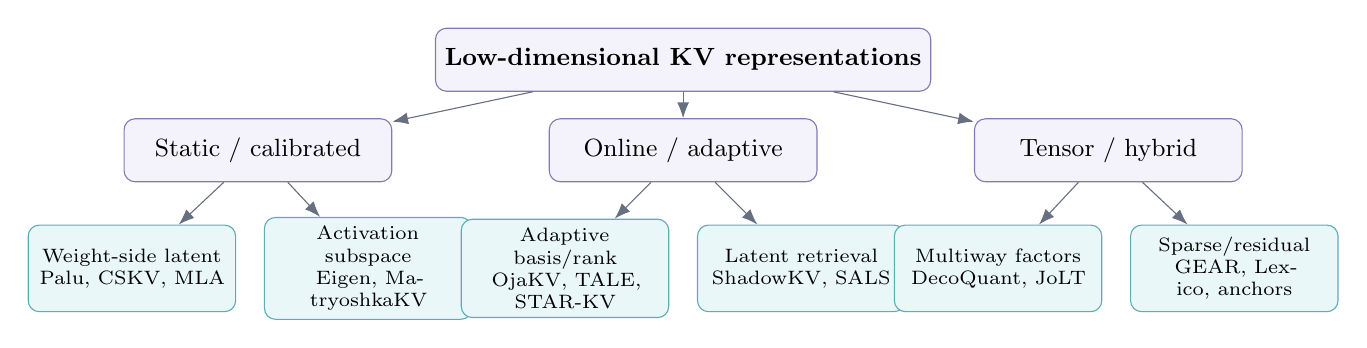
\begin{tikzpicture}[
 box/.style={rounded corners,draw=accent!65,fill=soft,align=center,minimum width=34mm,minimum height=8mm,font=\small},
 leaf/.style={rounded corners,draw=teal!65,fill=cool,align=center,text width=24mm,minimum height=11mm,font=\scriptsize},
 arr/.style={-{Latex[length=2mm]},draw=ink!65}
]
\node[box,minimum width=48mm] (root) at (0,0) {\textbf{Low-dimensional KV representations}};
\node[box] (static) at (-5.4,-1.15) {Static / calibrated};
\node[box] (online) at (0,-1.15) {Online / adaptive};
\node[box] (tensor) at (5.4,-1.15) {Tensor / hybrid};
\node[leaf] (weight) at (-7.0,-2.65) {Weight-side latent\\Palu, CSKV, MLA};
\node[leaf] (act) at (-4.0,-2.65) {Activation subspace\\Eigen, MatryoshkaKV};
\node[leaf] (oja) at (-1.5,-2.65) {Adaptive basis/rank\\OjaKV, TALE, STAR-KV};
\node[leaf] (sel) at (1.5,-2.65) {Latent retrieval\\ShadowKV, SALS};
\node[leaf] (ten) at (4.0,-2.65) {Multiway factors\\DecoQuant, JoLT};
\node[leaf] (res) at (7.0,-2.65) {Sparse/residual\\GEAR, Lexico, anchors};
\draw[arr] (root)--(static); \draw[arr] (root)--(online); \draw[arr] (root)--(tensor);
\draw[arr] (static)--(weight); \draw[arr] (static)--(act);
\draw[arr] (online)--(oja); \draw[arr] (online)--(sel);
\draw[arr] (tensor)--(ten); \draw[arr] (tensor)--(res);
\end{tikzpicture}
\end{center}

\subsection{Static activation-space projection}

\textbf{Eigen Attention} learns/calibrates low-rank subspaces and evaluates attention in the
reduced space. It established that feature reduction can lower both cache size and attention
latency, reporting up to 40\% cache reduction and 60\% attention-latency reduction
\cite{eigen}. Its limitation is a static subspace and a reconstruction-oriented proxy rather than
an objective tied to the final decoder output.

\textbf{MatryoshkaKV} learns orthogonal projections with nested usable ranks, allowing ranks to
vary across heads and layers without training a separate basis for each budget \cite{matryoshka}.
This makes allocation flexible, but still relies on trained static feature spaces.
\textbf{StiefAttention} directly attacks the objective mismatch by optimizing orthonormal bases
on a Stiefel manifold to minimize decoder-layer output error, then builds layerwise error--rank
profiles \cite{stief}. It is a strong 2026 preprint baseline for any ``attention-aware'' claim.
\textbf{Swift-SVD}, accepted at ICML 2026, gives an activation-aware closed-form spectral solution,
incremental covariance aggregation, and dynamic rank allocation for joint weight/KV reduction
\cite{swiftsvd}; it is a particularly strong calibration-time matrix baseline.

\textbf{KQ-SVD} argues that approximating keys alone is not optimal for preserving the attention
matrix and gives a closed-form decomposition targeting query--key interactions \cite{kqsvd}.
\textbf{CurDKV}, although it retains selected rows rather than storing factors, uses CUR leverage
scores and value information to preserve attention output; it shows why attention scores alone are
an insufficient importance target \cite{curdkv}. Together these works shift the standard from raw
Frobenius error toward attention or decoder-output fidelity.

\subsection{Weight-side and ``born compressed'' representations}

\textbf{Palu} factorizes key/value projection weights so low-dimensional latent states are cached;
its kernel work demonstrates the importance of fusing projections rather than reconstructing the
cache \cite{palu}. \textbf{LoRC} similarly performs post-training weight-level factorization, but
allocates layerwise sensitivity progressively because errors accumulate through depth
\cite{lorc}. \textbf{CSKV} uses low-rank K/V layers, a small exact recent branch, and lightweight
reconstruction training; it reports 80\% cache reduction, and up to 95\% when combined with
quantization \cite{cskv}.

\textbf{DeepSeek-V2's Multi-head Latent Attention (MLA)} is architectural rather than a retrofit:
the model is trained to cache a compact latent vector and separates positional information where
needed; DeepSeek-V2 reports 93.3\% KV-cache reduction relative to its stated comparison
\cite{mla}. \textbf{MHA2MLA} retrofits existing MHA models using joint SVD and partial RoPE with a
small amount of adaptation data, reporting 92.19\% reduction on Llama-2-7B with a 0.5\% LongBench
drop \cite{mha2mla}. These methods make a central feasibility point: the cheapest runtime
decomposition is often the one moved into fixed weights, but RoPE must be explicitly separated,
aligned, or otherwise handled.

\textbf{RAP} takes that lesson further: it prunes RoPE-aligned column pairs so transformations can
be absorbed and reconstruction eliminated \cite{rap}. It is pruning rather than a data-adaptive
factorization, but it closes off vague novelty claims based only on ``RoPE-aware low rank.''
\textbf{EliteKV} selects head-specific RoPE frequencies and applies joint low-rank K/V projection
with limited uptraining, reporting 75\% cache reduction in its tested model families
\cite{elitekv}.
\textbf{ReCalKV} differentiates K and V, reorders similar key heads for grouped SVD, and fuses the
value-side calibrated matrices to avoid added compute \cite{recalkv}.

\subsection{Online and token-adaptive low rank}

\textbf{TALE} makes ranks token-adaptive, compresses lazily, avoids key reconstruction by treating
K and V asymmetrically, and combines the representation with multilevel quantization. It reports
9.1$\times$ memory compression and up to 2$\times$ latency reduction in its long-context setting
\cite{tale}. \textbf{OjaKV} keeps crucial tokens as exact anchors and adapts the low-rank basis via
Oja's online PCA, with a larger prefill update and lightweight periodic decode updates
\cite{ojakv}. \textbf{STAR-KV} is a 2026 preprint using differentiable thresholding for adaptive
head/block ranks, hybrid K/V factorization, mixed precision, and Triton kernels \cite{starkv}.
\textbf{VarRate}, a very recent preprint, argues for variable-rate codes rather than uniform rank
or irreversible eviction \cite{varrate}.

The lesson is not that online fitting is always best. It is that a static basis can fail under
distribution shift, while per-token or per-block adaptation can cost more than it saves. Every
online proposal therefore needs an explicit \term{amortization horizon}: how many future reads
remain after a block is compressed?

\subsection{Low rank as an index for sparse retrieval}

\textbf{ShadowKV} keeps a low-rank key representation on GPU, offloads values, and reconstructs
only selected sparse KV pairs; it reports up to 6$\times$ larger batch sizes and 3.04$\times$
throughput on its A100 evaluations \cite{shadowkv}. \textbf{SALS} performs RoPE-free sparse token
selection in a low-rank latent space and reconstructs only the chosen tokens, reporting
6.4$\times$ cache compression and substantial operator/end-to-end gains in its settings
\cite{sals}. \textbf{RocketKV} combines coarse eviction with top-$k$ sparse attention and
low-dimensional selection \cite{rocketkv}. These systems use low rank primarily to reduce the
cost of \emph{finding} important tokens, not necessarily as the final representation from which
all attention is computed.

\subsection{Tensor decompositions and structured residuals}

\textbf{DecoQuant} uses matrix-product-operator/tensor decomposition to isolate outlier-bearing
small tensors and make the large tensors easier to quantize; the decomposition assists
data-free low-bit compression rather than defining direct tensor attention \cite{decoquant}.
\textbf{JoLT} is the closest tensor prior: a partial Tucker decomposition compresses token and
feature modes while leaving head/layer axes intact, and a Johnson--Lindenstrauss-rotated low-bit
residual recovers discarded energy. It reports near-lossless 2--3$\times$ compression and a
randomized variant that reduces compression time \cite{jolt}. \textbf{Tucker-KV} publicly proposed
HOSVD/HOOI refinement and budget allocation, but its ICLR 2026 submission was desk-rejected;
it is prior art, not peer-reviewed evidence \cite{tuckerkv}.

\textbf{GEAR} is the decisive prior for low-rank+sparse claims. It first quantizes most cache
entries, then approximates quantization error with a low-rank matrix and corrects individual
outliers with a sparse matrix \cite{gear}. \textbf{Lexico} represents each KV vector by sparse
coefficients over a universal dictionary, retaining 90--95\% of original GSM8K performance using
15--25\% of native cache memory in reported experiments \cite{lexico}. These works show that
residual structure matters, but leave open whether a \emph{tensor} bulk plus
\emph{attention-influence-structured} sparse residual can be executed directly.

\subsection{Diagnostics, negative evidence, and evaluation}

\textbf{KV-CoRE} benchmarks data-dependent rank compressibility across layers/domains and relates
normalized effective rank to downstream degradation \cite{kvcore}. \textbf{Quantization Dominates
Rank Reduction}, an unreviewed 2026 preprint, reports that at matched storage low-bit quantization
outperforms rank reduction across its tested models; its explanation is that projection can change
attention routing while bounded quantization often preserves dimension-wise information
\cite{quantdom}. Even if its universality is disputed, it sets the correct baseline challenge:
tensor/low-rank methods must beat INT4 at matched \emph{physical bytes}, not just beat SVD.

\textbf{The Risk of KV Cache Compression} studies intrinsic compressibility and worst-case risk
\cite{riskkv}. \textbf{The Pitfalls of KV Cache Compression} finds uneven instruction degradation
and system-prompt leakage under several eviction methods \cite{pitfalls}; it motivates protected
instructions and multi-instruction evaluation for all compression families. A workload-aware 2026
benchmark finds that compression ratio alone poorly predicts quality or end-to-end performance
\cite{benchmark}. The TMLR survey on KV-cache management likewise finds that method choice depends
on workload and system constraints \cite{survey}.

\section{Landscape table}

\footnotesize
\setlength{\LTpre}{2pt}\setlength{\LTpost}{4pt}
\renewcommand{\arraystretch}{1.15}
\begin{longtable}{@{}P{1.95cm}P{.9cm}P{2.5cm}P{2.55cm}P{2.75cm}P{2.7cm}@{}}
\toprule
\textbf{Method} & \textbf{Year} & \textbf{Main representation} &
\textbf{Adaptation / exact part} & \textbf{Execution idea} & \textbf{What remains open} \\
\midrule
\endfirsthead
\toprule
\textbf{Method} & \textbf{Year} & \textbf{Main representation} &
\textbf{Adaptation / exact part} & \textbf{Execution idea} & \textbf{What remains open} \\
\midrule
\endhead
Eigen Attention & 24 \pub & calibrated low-rank subspace & static, layer/head subspaces &
attention in reduced space & distribution shift; output-aware objective \\
GEAR & 24 \pub & quantized bulk + low-rank error + sparse outliers & online cache coding &
hybrid reconstruction/compute & attention-aware structured sparsity \\
CSKV & 24 \pub & low-rank K/V layers & small full-precision window & low-dimensional cache;
light training & direct tensor representation \\
DecoQuant & 24 \pub & MPO-assisted quantization & data-free transform & quantized tensors &
runtime factor-domain attention \\
LoRC & 24 \pre & weight low rank & progressive layer allocation & plug-in projection &
data-adaptive residual \\
DeepSeek MLA & 24 \pre & trained latent KV & decoupled positional branch & born compressed,
absorbed projections & retrofit without broad tuning \\
MHA2MLA & 25 \pub & joint K/V low rank + partial RoPE & data-efficient retrofit & converts
MHA/GQA toward MLA & adaptation data and deployment kernels \\
EliteKV & 25 \pre & RoPE frequency selection + joint low rank & limited uptraining & partially
restores key linearity & model-family transfer and kernel cost \\
Palu & 25 \pub & factorized K/V weights & calibrated grouping & fused latent computation &
adaptive per-input correction \\
MatryoshkaKV & 25 \pub & nested orthogonal projections & trainable rank choices & reduced
feature cache & runtime distribution shift \\
TALE & 25 \pub & token-adaptive low rank + quantization & lazy; K/V asymmetric & reconstruction
elimination & multiway/tensor residuals \\
ShadowKV & 25 \pub & low-rank keys + offloaded values & sparse selected tokens exact &
selective reconstruction & single-device no-offload direct path \\
SALS & 25 \pub & latent low rank for sparse selection & reconstruct selected tokens &
RoPE-free latent retrieval & all-token factor execution \\
RocketKV & 25 \pub & low-dim sparse retrieval & two-stage selection & top-$k$ attention &
representation fidelity of unselected tail \\
Lexico & 25 \pub & sparse universal dictionary & per-token OMP codes & sparse reconstruction &
cost of coding; low-rank bulk synergy \\
CurDKV & 25 \pub & CUR row selection & value-guided leverage & keeps selected KV exact &
direct low-rank/tensor storage \\
KQ-SVD & 25 \pre & attention-matrix low rank & query calibration & closed-form target &
runtime and tensor extension \\
OjaKV & 26 \pub & online PCA basis + anchors & prefill + periodic Oja updates & FlashAttention
compatible & update payback; tensor factors \\
StiefAttention & 26 \pre & Stiefel orthogonal bases & decoder-output calibration & static
compressed cache & online residual and kernels \\
Swift-SVD & 26 \pub & activation-aware spectral low rank & covariance aggregation + rank
allocation & training-free weight/KV reduction & matrix objective; no sparse tensor tail \\
RAP & 26 \pre & RoPE-pair column pruning & static & absorbed, no reconstruction & data-adaptive
bulk/residual coding \\
STAR-KV & 26 \pre & adaptive low rank + mixed precision & head/block thresholds & Triton path &
independent reproduction; sparse innovations \\
KV-CoRE & 26 \pre & rank diagnostic/benchmark & data/domain dependent & incremental SVD analysis &
policy using diagnostics online \\
Quant.\ Dominates & 26 \pre & matched-byte comparison & none & evaluation critique &
test tensor+sparse direct methods \\
JoLT & 26 \pre & partial Tucker + low-bit JL residual & joint rank/bit allocation &
fast randomized fitting & direct attention; longer payback study \\
Tucker-KV & 26 \unpub & Tucker HOSVD/HOOI & refinement and budgeting & representation study &
not archival; no novelty by Tucker alone \\
VarRate & 26 \pre & variable-rate low rank & token/block rate control & training-free policy &
independent reproduction and kernels \\
\bottomrule
\end{longtable}
\normalsize

\section{What the literature establishes---and what it does not}

\begin{center}
\small
\renewcommand{\arraystretch}{1.18}
\begin{tabularx}{.98\textwidth}{@{}p{3.1cm}X X@{}}
\toprule
\textbf{Question} & \textbf{Evidence-supported answer} & \textbf{Unresolved part} \\
\midrule
Is KV low rank? & Often, but unevenly across K/V, layers, heads, prompts, domain, and RoPE
placement. & No universal rank; an online policy must detect non-compressible blocks. \\
Does smaller storage mean faster decode? & Only when fewer HBM bytes are read and
reconstruction/update overhead is controlled. & Kernel crossover depends on rank, $S$, batch,
head type, layout, and hardware. \\
Static or online? & Static/weight-side is cheaper; online bases better track distribution shift. &
The best split between a fixed bulk and cheap online correction. \\
Frobenius or task-aware loss? & Attention/output-aware objectives better match model behavior. &
A cheap causal estimator of future-query influence. \\
Matrix or tensor? & Multiway axes offer structure, but Tucker/CP/TT overhead can erase the gain. &
Which modes are actually compressible and directly executable. \\
Low rank or quantization? & Quantization is a mandatory strong baseline and can dominate simple
rank reduction at matched bytes. & Whether structured tensor+sparse methods create a new Pareto
point at high dimension/long context. \\
\bottomrule
\end{tabularx}
\end{center}

\begin{gapbox}[title={Six defensible research gaps}]
\begin{enumerate}[leftmargin=1.55em,itemsep=3pt,topsep=2pt]
\item No established method combines a CP-structured multiway bulk with a \emph{RoPE-pair}
group-sparse error chosen by predicted attention-output influence.
\item Existing residual hybrids largely minimize entrywise, quantization, or energy error; they do
not cheaply optimize the risk of changing softmax routing under future queries.
\item Tensor papers focus primarily on representation/fitting; direct factor-domain attention and
end-to-end kernel crossover remain underdeveloped.
\item Online low-rank work adapts bases or ranks, but rarely makes compression admission depend on
the number of future cache reads needed to recover the fit cost.
\item K and V have different roles and spectra, yet many decompositions use symmetric modes,
ranks, residual criteria, and precision.
\item Evaluation still over-rewards nominal compression. Physical bytes, metadata, fit cost,
bytes/token, TPOT, energy, instruction preservation, and same-byte INT4 comparisons are often not
reported together.
\end{enumerate}
\end{gapbox}

\section{Recommended flagship: SAGE-CP-KV}

\begin{methodbox}[title={Softmax-Aware Group-sparse Error-corrected CP KV cache}]
\textbf{SAGE-CP-KV} stores the stable bulk of each old KV block as CP factors whose modes correspond
to token, KV head, RoPE frequency pair, and pair component. It stores only a small set of
attention-critical residual \emph{groups} aligned to complete RoPE pairs. A fused kernel computes
logits and value aggregation directly from CP coefficients and sparse groups. A recent exact
window protects local reasoning, and a payback controller uses native INT4 whenever tensor fitting
would not recover its cost.
\end{methodbox}

\subsection{Why this is the best first paper}

The idea has a clear Technique-Paper identity and a stronger novelty boundary than ``runtime
Tucker'':

\begin{itemize}[leftmargin=1.5em,itemsep=2pt]
\item It uses genuine multiway structure rather than replacing SVD with another dense
factorization.
\item It differs from GEAR: the sparse term corrects \emph{attention influence} in RoPE-pair
groups, not scalar quantization outliers.
\item It differs from JoLT: the bulk is CP with direct attention algebra, while the residual is
sparse and routing-aware rather than a dense low-bit JL residual.
\item It differs from SALS/ShadowKV: sparsity represents approximation failures, not merely a
selected token subset requiring reconstruction/offload.
\item It is more feasible than fully online robust tensor decomposition because the CP dictionary
can be calibrated offline and only token coefficients plus a tiny residual are computed online.
\end{itemize}

\subsection{Representation}

For an aged block of $n$ tokens, reshape each layer cache as
\[
\mathcal K,\mathcal V\in\R^{n\times H_{\mathrm{kv}}\times P\times 2},\qquad P=d/2,
\]
where the last two modes preserve complete RoPE pairs. Use separate CP ranks $R_K,R_V$:
\[
\widehat{\mathcal K}_{s,h,p,u}
=\sum_{r=1}^{R_K} A^K_{s,r}B^K_{h,r}C^K_{p,r}D^K_{u,r}+S^K_{s,h,p,u},
\]
\[
\widehat{\mathcal V}_{s,h,p,u}
=\sum_{r=1}^{R_V} A^V_{s,r}B^V_{h,r}C^V_{p,r}D^V_{u,r}+S^V_{s,h,p,u}.
\]
$B,C,D$ are calibrated per layer or layer group. Only token coefficients $A_{s,:}$ and sparse
residual groups grow with context. $S$ is group sparse over $(s,h,p)$ and always retains both
components $u\in\{0,1\}$, preserving RoPE-pair geometry and enabling regular memory access.
K and V may use different ranks, precision, and residual budgets.

\subsection{Softmax-aware fitting and sparse innovations}

Plain CP-ALS minimizes tensor Frobenius error, which can spend rank on harmless energy while
missing a small perturbation that changes attention routing. Calibrate CP factors using recorded
queries $\mathcal Q_\ell$ and a mixed objective
\[
\begin{split}
\min_{\Theta,S}\quad
&\E_{q\sim\mathcal Q_\ell}
 \norm{\Attn(q,\mathcal K,\mathcal V)
 -\Attn(q,\widehat{\mathcal K},\widehat{\mathcal V})}_2^2\\
&+\lambda_K\norm{\mathcal K-\widehat{\mathcal K}}_F^2
 +\lambda_V\norm{\mathcal V-\widehat{\mathcal V}}_F^2
 +\tau_K\norm{S^K}_{2,0,\mathrm{pair}}
 +\tau_V\norm{S^V}_{2,0,\mathrm{pair}} .
\end{split}
\]
For online residual admission, use a cheap upper-bound score rather than rerunning the full model.
Let $e^K_{s,h,p,:}$ and $e^V_{s,h,p,:}$ be a candidate pair residual, $\bar q_{h,p}$ a high
quantile of calibration-query magnitude, and $\bar\alpha_{s,h}$ predicted/observed attention mass:
\[
 I_{s,h,p} =
 c_K\,\bar\alpha_{s,h}\,\bar q_{h,p}\norm{e^K_{s,h,p,:}}_2
 +c_V\,\bar\alpha_{s,h}\norm{e^V_{s,h,p,:}}_2 .
\]
Store the highest-$I$ groups under a byte budget. A conservative floor always protects system
instructions, delimiters, exact numbers/entities identified by a lightweight policy, and the
recent window. The paper should call $I$ an \emph{influence surrogate}, not a proof of semantic
importance.

\subsection{Reconstruction-free attention algebra}

For query head $h$ and its associated KV head, define
\[
 Z^K_{h,r}(q)=B^K_{h,r}\sum_{p,u}q_{h,p,u}C^K_{p,r}D^K_{u,r}.
\]
Then every old-token logit is
\[
 \ell_{s,h}=\frac{1}{\sqrt d}\left(
\sum_r A^K_{s,r}Z^K_{h,r}(q)
+ \sum_{(p,u)\in\Omega^K_{s,h}}q_{h,p,u}S^K_{s,h,p,u}
\right).
\]
This reads an $n\times R_K$ coefficient matrix plus compact factors, not an $n\times d$ key
matrix. After online softmax produces $\alpha_{s,h}$, first reduce over tokens,
\[
 g^V_{h,r}=\sum_s\alpha_{s,h}A^V_{s,r},
\]
then form the current output vector
\[
 o_{h,p,u}=\sum_r g^V_{h,r}B^V_{h,r}C^V_{p,r}D^V_{u,r}
+\sum_s\alpha_{s,h}S^V_{s,h,p,u}.
\]
Only the current $d$-dimensional output is formed; no dense old-$V$ cache is reconstructed.
Blockwise log-sum-exp merges exact-hot, CP, sparse, and fallback INT4 blocks.

\subsection{Feasible lifecycle and computation cost}

\begin{enumerate}[leftmargin=1.55em,itemsep=3pt]
\item \textbf{Offline calibration:} learn $B,C,D$, ranks, query statistics, and optionally a
small coefficient encoder. This absorbs expensive CP optimization before deployment.
\item \textbf{Native hot window:} append recent K/V in BF16, FP8, or INT4. Do not factorize per
token and do not alter the just-produced layer output.
\item \textbf{Age-triggered coding:} when a block leaves the window, compute $A$ with a
precomputed regularized pseudoinverse or a one-pass encoder; compute residual pair scores and keep
top groups. A bounded one-iteration refinement is an ablation, not a dependency.
\item \textbf{Payback admission:} let $C_{\mathrm{fit}}$ be measured coding time, $\Delta t$ the
measured time saved per future decode read, and $N_{\mathrm{future}}$ a conservative remaining
decode estimate. Admit CP coding only if
\[
N_{\mathrm{future}}\Delta t > C_{\mathrm{fit}}+C_{\mathrm{margin}}.
\]
Otherwise retain the block in the fastest available native/INT4 representation.
\end{enumerate}

\begin{keybox}[title={Intuitive advantage}]
CP factors capture the repeated, globally shared structure across heads and frequency pairs;
sparse innovations preserve rare local exceptions such as names, numbers, delimiters, and
instruction-bearing features. Pair grouping respects RoPE and maps to contiguous GPU work.
Direct factor attention turns representation compression into fewer HBM bytes per token. The
payback gate prevents the common failure where a beautiful decomposition makes inference slower.
\end{keybox}

\subsection{Memory model and target operating region}

Ignoring amortized fixed factors, dense BF16 storage per token/layer is
$4H_{\mathrm{kv}}d$ bytes. SAGE-CP-KV stores approximately
\[
 2b_A(R_K+R_V)+m_K(2b_S+b_I)+m_V(2b_S+b_I)
\]
bytes per token/layer, where $m_K,m_V$ are retained RoPE-pair groups and $b_I$ includes compressed
indices. Fixed CP factors and rank tables must be included in measured allocation. The first
target should be a conservative 4--8$\times$ physical reduction with near-full task quality,
not a maximal nominal ratio.

\subsection{Theory targets}

For bounded quantities and approximation errors
\[
\norm{q}_2\le Q,\qquad \max_s\norm{V_s}_2\le M_V,\qquad
\epsilon_K=\max_s\norm{K_s-\widehat K_s}_2,\qquad
\epsilon_V=\max_s\norm{V_s-\widehat V_s}_2,
\]
softmax Lipschitzness gives a target bound of the form
\[
\norm{\Attn(q,K,V)-\Attn(q,\widehat K,\widehat V)}_2
\le c_{\mathrm{sm}}\frac{Q\epsilon_K}{\sqrt d}M_V+\epsilon_V ,
\]
with constants and norm choices stated precisely in the paper. The stronger contribution is a
group-selection result: under a calibrated query envelope, selecting the largest influence-bound
groups minimizes the stated separable upper bound at a fixed group budget. Do not claim global
optimality for CP rank or future-query prediction.

\subsection{Experiments that can support publication}

\small
\renewcommand{\arraystretch}{1.16}
\begin{longtable}{@{}P{2.6cm}P{8.35cm}P{3.1cm}@{}}
\toprule
\textbf{Claim} & \textbf{Experiment} & \textbf{Pass criterion before writing the claim} \\
\midrule
\endfirsthead
\toprule
\textbf{Claim} & \textbf{Experiment} & \textbf{Pass criterion before writing the claim} \\
\midrule
\endhead
Multiway structure exists & CP rank/conditioning curves on recorded post-RoPE K and V by layer,
head type, context, and domain & Stable rank gives $\ge4\times$ physical reduction on substantial
layers \\
Sparse tail protects routing & Compare no residual, magnitude scalar, random pair, energy pair,
and influence pair at equal bytes & Influence pairs improve attention-output and downstream
quality consistently \\
Direct execution is real & Explicit reconstruction vs factor kernel vs FlashAttention/INT4
microbenchmarks & No old dense allocation; positive latency region at realistic $S,B$ \\
Online cost is repaid & Report fit time and future-read crossover per block & Controller declines
unprofitable cases and amortized overhead stays small \\
Quality is robust & LongBench, RULER, GSM8K/MATH, PG-19 or WikiText; multi-instruction IFEval and
prompt-leakage checks & Near-full quality at the selected operating point across two model families \\
New Pareto point & Same physical bytes against KIVI/INT4, Palu, Eigen, TALE, OjaKV, SALS,
Lexico, GEAR, JoLT & Better quality or TPOT at equal memory on at least one important regime,
without hiding regressions \\
\bottomrule
\end{longtable}
\normalsize

Recommended models are one GQA family (Llama-3.1/3.2 or Qwen2.5/3) and one MHA or different-GQA
family (Mistral/Llama-2), subject to license and hardware. Sweep context 2K--128K where feasible,
batch size, hot-window length, $R_K/R_V$, sparse budget, precision, and pre/post-RoPE coding.
Report TTFT, TPOT, tokens/s, peak allocation, actual cache bytes, metadata, bytes read/token,
fit time, energy/token, and accuracy. Use bootstrap confidence intervals or repeated seeds for
task metrics.

\begin{riskbox}[title={Fatal-flaw gates}]
\begin{itemize}[leftmargin=1.45em,itemsep=2pt,topsep=2pt]
\item If CP rank is high or unstable on values, pivot to CP keys + quantized values; do not force a
symmetric method.
\item If factor kernels do not beat INT4 at long context, publish only if the quality-at-memory
gain is large and honestly position it as a capacity method.
\item If influence selection does not beat pair magnitude at equal bytes, the claimed novelty is
not supported.
\item If online coefficient/residual coding cannot repay itself, move coding to prefill/offline
weight-side generation or abandon runtime fitting.
\item If gains disappear on a second model/domain, narrow the claim to a diagnosed compressibility
regime rather than claiming universal KV structure.
\end{itemize}
\end{riskbox}

\section{Shared mathematical foundation of the proposed portfolio}

All four ideas use the same high-dimensional modeling principle but apply it to different
objects and system boundaries. For a $D$-way tensor
$\mathcal X\in\R^{n_1\times\cdots\times n_D}$, we seek
\[
\mathcal X=\mathcal L+\mathcal S+\mathcal E,
\qquad
\text{structured rank}(\mathcal L)\ \text{small},\quad
\norm{\mathcal S}_{2,0,\mathcal G}\le k,\quad
\norm{\mathcal E}\le\varepsilon ,
\]
where $\mathcal L$ captures recurring global structure, $\mathcal S$ contains a small number
of exceptional groups from a hardware-aligned partition $\mathcal G$, and $\mathcal E$ is the
unrepresented tail. This is a modeling hypothesis to be tested per layer, prompt, and modality,
not assumed universally.

\subsection{Three tensor representations under consideration}

\begin{itemize}[leftmargin=1.55em,itemsep=3pt]
\item \textbf{CP:}
\[
\mathcal L_{i_1,\ldots,i_D}
=\sum_{r=1}^{R}\prod_{d=1}^{D}U^{(d)}_{i_d,r},
\qquad
\bytes(\mathcal L)=b\sum_{d=1}^{D}n_dR.
\]
CP has the smallest and most direct factor algebra, which is why it is the first choice for
SAGE-CP-KV. Its main difficulty is numerical conditioning and the possible nonexistence of a
stable best rank-$R$ approximation.
\item \textbf{Tucker:}
\[
\mathcal L=\mathcal G\times_1 U^{(1)}\times_2\cdots\times_D U^{(D)},\qquad
\bytes(\mathcal L)=b\left(\prod_d r_d+\sum_dn_dr_d\right).
\]
Tucker provides separate ranks per semantic mode and is often easier to fit, but the core
$\mathcal G$ can grow exponentially with the number of jointly compressed modes. JoLT already
occupies much of the direct Tucker novelty space.
\item \textbf{Tensor Train:}
\[
\mathcal L_{i_1,\ldots,i_D}
=G^{(1)}[:,i_1,:]G^{(2)}[:,i_2,:]\cdots G^{(D)}[:,i_D,:],
\qquad
\bytes(\mathcal L)=b\sum_{d=1}^{D}r_{d-1}n_dr_d,
\]
with $r_0=r_D=1$. TT is attractive for causal/multiscale token tensorization and for
LoSpar-CI/CATT-KV, but ranks can grow under appends, permutations, or poorly chosen mode order.
\end{itemize}

The sparse term is deliberately \emph{group} sparse rather than arbitrarily element sparse:
\[
\norm{\mathcal S}_{2,0,\mathcal G}
=\sum_{g\in\mathcal G}\mathbf 1\{\norm{\mathcal S_g}_2>0\}.
\]
Candidate groups include RoPE coordinate pairs, feature tiles, tokens, attention heads, spatial
patches, or hyperspectral bands. Grouping slightly reduces the ideal compression ratio but makes
the representation semantically meaningful and executable by regular GPU/edge kernels.

\begin{keybox}[title={Why low rank and sparsity are complementary}]
Low rank explains the \emph{shared bulk}: correlations repeated across tokens, heads, frequency
pairs, spatial patches, or devices. Sparsity explains \emph{rare innovations}: prompt-specific
entities, numbers, instructions, pathological regions, unusual spectral signatures, and
distribution-shift errors that a fixed subspace misses. Low rank alone can blur rare information;
sparsity alone repeatedly stores common structure. Their combination is useful only when the
sparse support remains small and the factor/residual kernels are cheaper than dense movement.
\end{keybox}

\section{LoSpar-CI: progressive tensor factors plus sparse refinement}

\begin{methodbox}[title={Proposed cross-domain technique}]
\textbf{LoSpar-CI} proposes to transmit the intrinsic structure of a high-dimensional intermediate
tensor across collaborating devices: send tensor factors for a coarse low-rank component first,
then request sparse innovation groups only while the downstream decision is not certifiably stable.
\end{methodbox}

\subsection{Intended setting and research gap}

The strongest LoSpar-CI setting is not batch-1 LLM decode activation transfer; a single token
crossing a pipeline boundary is only one hidden vector and its network cost may be dominated by
round-trip/framework latency. The natural setting is an actually high-dimensional boundary tensor:
long-prompt prefill activations, hyperspectral cubes, dynamic MRI/CT, long video, 3D volumes, or
whole-slide-image features. Robust PCA and tensor decompositions provide the mathematical
foundation for low-rank-plus-sparse structure \cite{rpca,kolda,tt}; HexGen, Jupiter, and the
FSU edge-pipeline poster provide the collaborative-inference setting
\cite{hexgen,jupiter,poster}.

\subsection{Representation and communication complexity}

At pipeline cut $\ell$, let
\[
\mathcal A_\ell=\mathcal L_\ell+\mathcal S_\ell+\mathcal E_\ell,\qquad
\norm{\mathcal E_\ell}\le\varepsilon_0.
\]
For a TT implementation, device $d_p$ transmits cores
$\{G_\ell^{(j)}\}_{j=1}^{D}$ at cost
\[
C_L=b_L\sum_{j=1}^{D}r_{j-1}n_jr_j .
\]
Let $k$ of $N_G$ fixed-size groups be retained in $\mathcal S_\ell$. A direct support/value
code costs approximately
\[
C_S(k)=k\,b_{\mathrm{group}}+
\left\lceil\log_2 \binom{N_G}{k}\right\rceil
\ \lesssim\ k\,b_{\mathrm{group}}+
k\log_2\!\left(\frac{eN_G}{k}\right).
\]
The total is $C_L+C_S(k)$ rather than $b\prod_jn_j$, but only after factor headers, indices,
padding, quantization scales, and the cost of fitting $\mathcal L_\ell$ are counted.

\subsection{Progressive protocol and a correct decision certificate}

Let $\widehat{\mathcal A}^{(j)}_\ell=\widehat{\mathcal L}_\ell+
\mathcal S_\ell^{(j)}$ after $j$ sparse groups, and assume a computable residual bound
\[
\norm{\mathcal A_\ell-\widehat{\mathcal A}^{(j)}_\ell}\le\eta_j .
\]
Let $F_\ell$ map the cut activation to final logits and satisfy locally
\[
\norm{F_\ell(A)-F_\ell(A')}_\infty\le
\kappa_\ell\norm{A-A'}.
\]
If the approximate top-two logit margin is
$\widehat\mu_j=\widehat y_{(1)}-\widehat y_{(2)}$, then
\[
\widehat\mu_j>2\kappa_\ell\eta_j
\quad\Longrightarrow\quad
\arg\max F_\ell(\mathcal A_\ell)
=\arg\max F_\ell(\widehat{\mathcal A}^{(j)}_\ell).
\]
The factor two protects both the winning and runner-up logits. The sender transmits low-rank
factors first; the receiver stops if the inequality holds, otherwise it requests the next
highest-priority residual group. For generation, a strict global certificate is probably too
costly per token; there it should become an offline-calibrated error-budget allocator rather than
a repeated downstream recomputation.

\subsection{What would constitute the paper}

\begin{enumerate}[leftmargin=1.55em,itemsep=3pt]
\item A modality-specific demonstration that selected boundary tensors have stable TT/Tucker
rank plus a concentrated group-sparse tail.
\item A progressive factor/residual wire protocol with measured encoding, metadata, and
recomputation costs.
\item A certified or statistically calibrated early-stop rule that determines how many residual
groups each sample requires.
\item An end-to-end multi-device evaluation showing that bytes and latency scale with intrinsic
rank/sparsity rather than ambient tensor dimension.
\end{enumerate}

\begin{donebox}[title={Expected advantages}]
Communication can fall dramatically when ambient dimension grows while TT/Tucker ranks and
innovation count remain small. Progressive transmission adapts quality per example instead of
committing to one lossy compression ratio. The sparse tail protects rare, high-value information
that low rank tends to smooth away. A valid margin certificate provides a much stronger quality
story than an average reconstruction metric.
\end{donebox}

\begin{riskbox}[title={Possible limitations}]
The structural assumption can fail at some cuts, layers, or modalities; TT ranks and sparse
support may be too large. Tensor fitting can exceed the communication time saved. Lipschitz bounds
may be so loose that almost no sample stops early, and repeated refinement adds round trips.
For LLM batch-1 decoding, boundary-message size is often not the bottleneck. The first LoSpar-CI
paper should therefore choose one demonstrably compressible high-dimensional modality or prefill,
profile decomposition payback, and keep a dense fallback.
\end{riskbox}

\section{Shufflerless-CI: stationary latent--residual collaborative decoding}

\begin{methodbox}[title={Proposed systems co-design}]
\textbf{Shufflerless-CI} proposes to make KV state stationary on the device that owns each layer.
A fixed RoPE-safe low-rank projection creates the bulk cache, a sparse prompt-specific residual
corrects aged blocks, and a heterogeneous placement planner admits only requests whose weights,
cache, and workspace fit without CPU--GPU or inter-device KV movement.
\end{methodbox}

\subsection{Born-compressed bulk and online sparse innovations}

For layer $\ell$, factor projection weights offline:
\[
W^K_\ell\approx U^K_\ell(P^K_\ell)^\top,\qquad
W^V_\ell\approx U^V_\ell(P^V_\ell)^\top .
\]
For hidden state $x_s$, cache only
\[
z^K_s=x_sU^K_\ell,\qquad z^V_s=x_sU^V_\ell ,
\]
plus a small exact hot window. When a full block $B$ ages, compute once
\[
E_B^K=K_B-\widehat K_B(z_B^K),\qquad
E_B^V=V_B-\widehat V_B(z_B^V),
\]
retain hardware-aligned top-$k_{\ell h}$ innovation groups, and discard the dense block. This
avoids a per-token or accumulated-cache SVD. RoPE requires either complete coordinate-pair
projection, as motivated by RAP, or a small exact positional branch plus semantic latent, as in
MLA/MHA2MLA \cite{rap,mha2mla,mla}.

\subsection{Direct attention and exact hot/cold merge}

For a compatible factorization, the old-block score and value contribution have the form
\[
s_{tB}\approx (q_tP^K_\ell)(z_B^K)^\top+q_t(E_B^K)^\top,
\]
\[
\alpha_BV_B\approx
\big(\alpha_Bz_B^V\big)(P^V_\ell)^\top+\alpha_BE_B^V.
\]
The dense old $K_B,V_B$ are never allocated. Exact-hot and approximate-old segments produce
block statistics
\[
m_j=\max_s s_{js},\quad
\ell_j=\sum_s e^{s_{js}-m_j},\quad
o_j=\sum_s e^{s_{js}-m_j}v_{js}.
\]
Following online softmax/FlashAttention \cite{onlinesoftmax,flashattention}, their exact merge is
\[
m=\max_jm_j,\qquad
\ell=\sum_je^{m_j-m}\ell_j,\qquad
o=\sum_je^{m_j-m}o_j,\qquad
\operatorname{output}=o/\ell.
\]
This merge adds no approximation; all error is isolated to the compressed old-block
representation.

\subsection{Joint placement and deterministic no-shuffle admission}

For devices $i=1,\ldots,P$, the planner chooses the contiguous layer partition $\pi$, ranks
$r_\ell$, sparse budgets $k_\ell$, bit widths $b_\ell$, and hot windows $W_\ell$:
\[
\min_{\pi,r,k,b,W}\ \max_i T_i(\pi,r,k,b,W)
\]
subject to
\[
M_i^{\mathrm{weights}}(\pi)+M_i^{\mathrm{hot}}(W)
+M_i^{\mathrm{old}}(r,k,b)+M_i^{\mathrm{workspace}}\le M_i,
\]
\[
\sum_{\ell,h}\mathcal E_{\ell h}(r_{\ell h},k_{\ell h},b_{\ell h})
\le\epsilon .
\]
For an admitted maximum sequence length, these inequalities make ``no shuffle'' a deterministic
capacity property rather than a hope. The implementation must verify it with explicit-copy,
page-migration, page-fault, and synchronization traces, especially on unified-memory Jetsons.

\begin{donebox}[title={Expected advantages}]
The method directly targets the memory wall and tail latency: each layer reads a compact local
cache, never waits for remote KV, and never allocates a dense reconstruction buffer. Fixed
weight-side factors avoid runtime decomposition, while sparse innovations provide prompt-specific
adaptation. Joint rank/placement allocation can rebalance a heterogeneous pipeline and admit
longer contexts than the fixed dense partition.
\end{donebox}

\begin{riskbox}[title={Possible limitations}]
The decomposition primitives are close to Palu, Eigen Attention, RAP, OjaKV, and other hybrids;
novelty must come from the stationary representation--placement co-design and a decisive fixed-
versus-joint-placement ablation. Sparse indexing or RoPE processing may erase kernel gains.
A fixed subspace may fail under domain shift. Admission control can reject long or uncertain
requests rather than serving them. Finally, the project requires a multi-device implementation,
so it is less feasible as the first paper than SAGE-CP-KV.
\end{riskbox}

\section{SparsePipe: sparsity as a schedulable distributed resource}

\begin{methodbox}[title={Proposed adaptive systems layer}]
\textbf{SparsePipe} proposes to choose block sparsity, compression primitive, wire format, and
pipeline allocation jointly from live compute, bandwidth, memory, and quality state. It treats
sparsity as a runtime resource rather than a fixed model hyperparameter and always retains a
dense/exact fallback.
\end{methodbox}

\subsection{Mask prediction and joint control problem}

At boundary $p$ and control interval $t$, a lightweight predictor produces block scores
$a_{p,t}=g_{\theta_p}(x_{p,t})$ and the controller selects
\[
m_{p,t,g}=\mathbf1\{a_{p,t,g}\ge\tau_{p,t}\},
\qquad g=1,\ldots,N_{p}^{\mathrm{blk}}.
\]
The action $\sigma_t$ contains mask thresholds, token/KV budget, representation type, bit width,
wire format, and a \emph{coarse-timescale} partition choice. The optimization target is
\[
\min_{\sigma_t}\ 
\alpha\,\mathrm{TTFT}(\sigma_t)+\beta\,\mathrm{TPOT}(\sigma_t)
+\gamma\,\mathrm{Energy}(\sigma_t)+\delta\,\mathrm{Memory}(\sigma_t)
+\zeta\max_i\mathrm{Latency}_i(\sigma_t)
\]
subject to per-device memory and
\[
\operatorname{QualityRisk}(\sigma_t)\le\rho .
\]
The partition should not move every token: moving weights or KV would contradict the latency
goal. Fast control changes masks/formats; slow control changes partitions only between requests
or at rare safe synchronization points.

\subsection{A wire-format crossover that counts metadata}

If each block contains $G$ values of $b_v$ bytes, $N_{\mathrm{blk}}$ blocks exist, and
$n_a$ are active, then
\[
C_{\mathrm{dense}}=N_{\mathrm{blk}}Gb_v,\qquad
C_{\mathrm{sparse}}=n_aGb_v+C_{\mathrm{index}}(n_a,N_{\mathrm{blk}}).
\]
Sparse transmission is selected only when $C_{\mathrm{sparse}}<C_{\mathrm{dense}}$ and the
profiled sparse kernel plus packing time is faster. With a bitmap,
$C_{\mathrm{index}}=N_{\mathrm{blk}}/8$ bytes; with explicit indices it is approximately
$n_a\lceil\log_2N_{\mathrm{blk}}\rceil/8$. This simple crossover prevents the controller from
choosing ``sparsity'' that increases total traffic.

\subsection{Composed accuracy budget}

Suppose an approximation error $\Delta_p$ is injected at boundary $p$ and the downstream suffix
$F_{p+1:P}$ has local Lipschitz constant $\kappa_{p+1:P}$. For multiple boundaries,
\[
\norm{\Delta_{\mathrm{out}}}
\le \sum_{p=1}^{P-1}\kappa_{p+1:P}\norm{\Delta_p}.
\]
SparsePipe allocates a conservative error budget $\rho_p$ so that
$\sum_p\kappa_{p+1:P}\rho_p\le\rho$. Because worst-case constants can be loose, the deployable
version should combine calibrated empirical risk with exact fallback and report both the formal
bound and its coverage/tightness.

\subsection{How tensor and low-rank methods enter SparsePipe}

SparsePipe is a controller, not a replacement for SAGE-CP-KV or LoSpar-CI. Its action set can
select among dense, INT4, CP-only, CP+sparse, TT/Tucker factors, token eviction, or exact protected
storage. For high-dimensional prefill boundaries it can choose LoSpar-CI's factor/residual wire
format; for local KV it can choose SAGE-CP-KV; for the multi-device steady-state guarantee it can
respect Shufflerless-CI's stationary placement. This composability is the most defensible
positioning.

\begin{donebox}[title={Expected advantages}]
The method can respond to bandwidth drops, thermal throttling, queue changes, and heterogeneous
devices instead of using one compression ratio everywhere. Block granularity and format switching
make sparsity hardware-aware. Joint control can spend quality budget where it most reduces the
pipeline bottleneck, and exact fallback provides a safety floor. The controller can reuse advances
in tensor, quantization, eviction, or sparse coding as interchangeable actions.
\end{donebox}

\begin{riskbox}[title={Possible limitations}]
The scope is broad: token, neuron, attention, KV, wire format, and placement decisions can make
credit assignment and evaluation unwieldy. Contextual sparsity predictors can fail under shift,
and conservative quality bounds may force dense execution. At batch-1 decode, activation bytes
may be too small for sparsification to overcome network round-trip latency. Sparse kernels,
packing, and indices often cost more than idealized FLOP models suggest. Per-token repartitioning
is infeasible. SparsePipe should therefore begin with one or two actions, a profiled model-
predictive/bandit controller, and a static-sparsity plus fixed-partition ablation.
\end{riskbox}

\section{Portfolio comparison and recommended sequencing}

\small
\renewcommand{\arraystretch}{1.18}
\begin{longtable}{@{}P{2.25cm}P{2.35cm}P{2.5cm}P{2.65cm}P{2.65cm}P{2.15cm}@{}}
\toprule
\textbf{Idea} & \textbf{Compressed object} & \textbf{Tensor / low-rank role} &
\textbf{Sparse role} & \textbf{Primary advantage} & \textbf{Main limitation} \\
\midrule
\endfirsthead
\toprule
\textbf{Idea} & \textbf{Compressed object} & \textbf{Tensor / low-rank role} &
\textbf{Sparse role} & \textbf{Primary advantage} & \textbf{Main limitation} \\
\midrule
\endhead
SAGE-CP-KV & Old KV on one accelerator & CP across token/head/RoPE pair/component &
Influence-selected RoPE-pair corrections & Direct factor attention; strongest first-paper
balance & CP conditioning and kernel crossover \\
LoSpar-CI & High-dimensional boundary activation & TT/Tucker/CP factors transmitted first &
Progressive exceptional groups & Intrinsic-complexity communication with certificate &
Loose certificate; refinement/fitting overhead \\
Shufflerless-CI & Per-layer KV across an edge pipeline & Fixed born-compressed latent &
Aged-block prompt innovations & Deterministic stationary cache and lower tail latency &
Multi-device complexity; novelty is systems coupling \\
SparsePipe & Multiple runtime objects and formats & Selects tensor/latent codecs as actions &
Schedules block masks and exact fallback & Adapts to live heterogeneity and bandwidth &
Very broad scope; predictor/kernel overhead \\
\midrule
FD-KV & Streaming KV basis on one accelerator & Deterministic Frequent-Directions sketch of the
key stream, query-whitened & Optional attention-weighted V metric & Provable online basis at
fixed update cost; beats heuristic Oja & Tracks only the dominant subspace \\
SC-KV & Aged KV blocks on one accelerator & Union of low-rank subspaces (block-term) per token
cluster & Per-cluster residual groups & Captures multi-domain heterogeneity one subspace misses &
Cluster metadata; hard assignment needed for direct execution \\
\bottomrule
\end{longtable}
\normalsize

\begin{keybox}[title={Recommended sequence}]
\textbf{Phase 1:} test SAGE-CP-KV on recorded single-device KV and build the direct CP+sparse
kernel. \textbf{Phase 2:} if the kernel yields a real Pareto improvement, integrate it into
Shufflerless-CI and jointly optimize representation with the poster's layer partition.
\textbf{Parallel/alternative branch:} test LoSpar-CI on one genuinely high-dimensional modality
where $L+S+E$ is well supported. \textbf{Phase 3:} add SparsePipe only after two or more
representation choices have measured operating regions worth scheduling.
\end{keybox}

\section{Companion ideas, ranked}

\subsection{Idea 2: Payback-KV---a heterogeneous representation controller}

Choose per block among native FP16/FP8, INT4, CP-only, CP+sparse, and exact protected storage using
measured fit cost, predicted remaining output length, rank diagnostics, and kernel latency tables.
The contribution is a decision policy over \emph{realized latency and quality risk}, not another
compression format. It is highly feasible and systems-friendly, but its novelty is moderate unless
the controller has a principled regret/risk formulation and demonstrates broad hardware transfer.
Best fit: MLSys/ASPLOS/EuroSys; use it as a controller contribution around SAGE-CP-KV rather than a
standalone NeurIPS method initially.

\subsection{Idea 3: CATT-KV---causal Tensor-Train with sparse innovations}

Tensorize old token positions into dyadic causal digits and maintain SVD-free TT cores. Derive
RoPE-equivariant core contractions and store attention-critical sparse innovations. This can model
multiscale sequence structure better than CP and has the highest algorithmic upside. It is also
the riskiest: TT ranks may grow, appends and block merges are complex, and direct softmax still
needs all token logits unless combined with hierarchical screening. Pursue after the CP pilot shows
that tensor-domain execution has a positive crossover. Best fit if successful: NeurIPS/ICML for
the method plus MLSys/ASPLOS for a kernel-heavy version.

\subsection{Idea 4: protected-instruction tensor cache}

Use a learned or certified policy to route system instructions, delimiters, and low-frequency
semantic anchors to exact/sparse storage while factorizing ordinary context. The gap is motivated
by instruction-loss and prompt-leakage evidence \cite{pitfalls}. It becomes publishable only if the
protection rule generalizes beyond hand-written token classes and improves safety at matched bytes;
otherwise it is an evaluation ablation, not a full paper.

\subsection{Idea 5: distribution-shift-triggered tensor adaptation}

Keep offline CP factors but monitor a cheap residual/influence statistic. Only when it exceeds a
threshold, update a small factor subset or open new rank components; retire them when no longer
useful. This hybrid addresses the static-basis weakness identified by OjaKV without continuous
adaptation. The hard novelty question is whether the trigger and update outperform Oja's matrix
subspace at matched update cost. Treat this as a second paper or SAGE-CP-KV extension.

\subsection{Ideas 6--7: open-corner methods from the tensor-decomposition literature}

Two directions survive a strict novelty--feasibility--publishability filter against the surveyed
landscape; both target the open problems of \S4.1 (static-basis distribution shift,
Frobenius-versus-output-aware objective, K/V asymmetry) and the six gaps of \S6 using decomposition
machinery not yet applied to KV caches. They are added to the comparison table (\S12) and the
evaluation (\S14). Weaker corners are merged into them or explicitly not pursued (end of this
subsection).

\subsubsection*{Idea 6: FD-KV---a provable, output-aware streaming basis}

Replace the static subspace of \S4.1 (Eigen, MatryoshkaKV) and the heuristic online PCA of OjaKV
with a \term{Frequent-Directions} sketch \cite{fd_liberty,fd_ghashami}: per layer and KV head,
maintain an $\ell\times d$ sketch $B$ of the streaming key rows whose top-$r$ right singular
vectors form the compression basis. FD is deterministic and satisfies
$0\preceq K^\top K-B^\top B$ and $\norm{K^\top K-B^\top B}_2\le\norm{K-K_r}_F^2/(\ell-r)$---a
worst-case bound on the exact Gram/feature subspace attention projects onto, at fixed $O(d\ell)$
update cost, a guarantee Oja's stochastic-gradient PCA lacks. \emph{Two refinements make the
objective output-aware and K/V-asymmetric}, absorbing what would otherwise be a separate, weaker
idea: run FD on query-whitened key rows $qK$ so the bound becomes a score-fidelity bound
(\S6 gap~2), and sketch V in an attention-mass-weighted metric because $o=\sum_s\alpha_sV_s$
weights value error by attention (\S6 gap~5). \term{Closest prior:} OjaKV (online PCA, no
worst-case error), STAR-KV (soft-threshold ranks), and KQ-SVD (query-aware K, but offline and
matrix-only); the streaming-attention discrepancy sketch \cite{streamattn} is adjacent but targets
the attention product, not a cached basis. \term{Novelty:} a deterministic, guaranteed,
query-whitened streaming KV basis with asymmetric K/V metrics at matched update cost---the
comparison Idea~5 calls unresolved. \term{Feasibility:} very high (a few lines; no offline
calibration required). \term{Falsification:} FD-basis versus Oja versus static SVD under domain
shift, at equal bytes and equal update cost. \term{Risk:} it tracks only the dominant subspace and
degrades---rather than fails---when KV is genuinely high rank.

\subsubsection*{Idea 7: SC-KV---subspace-clustered KV via block-term decomposition}

A single global low-rank subspace blurs the heterogeneity that makes ``no universal rank'' true
(\S6 Q\&A). Model each aged block as a \term{union of low-rank subspaces}---a block-term
decomposition \cite{btd} with rank-$(L,L,1)$ terms---by clustering old tokens into a few groups
and giving each group its own small subspace. With a \emph{hard} token-to-cluster assignment this
is directly executable: per-cluster scores come from per-cluster factors and merge by the same
online-softmax argument used elsewhere, with no dense reconstruction. It addresses distribution
shift \emph{representationally} (complementary to FD's temporal adaptation) and the ``which modes
are compressible'' question (gap~3, \S4.1). \term{Closest prior:} every \S4.1 method and
xKV/OjaKV fit \emph{one} subspace per head/layer; no surveyed KV method uses a block-term or
union-of-subspaces representation. \term{Feasibility:} moderate---$k$-means on keys plus
per-cluster SVD is easy offline, but online cluster assignment, metadata, and block kernels need
care. \term{Falsification:} on a long multi-section prompt, do $k$ subspaces of rank $r/k$ beat one
rank-$r$ subspace at equal bytes on attention-output error? \term{Risk:} cluster-boundary metadata
and assignment cost; keep assignments hard to preserve direct execution.

\subsubsection*{Merged and not-pursued corners}

\textbf{Merged.} A fast randomized coefficient solve (TensorSketch \cite{tensorsketch}) is not a
representation but a fit-cost \emph{enabler}; fold it into the SAGE-CP-KV / SC-KV online coding
step to help the payback gate clear (\S6 gap~4) rather than ranking it. The query-whitened K and
attention-weighted V metrics are merged into FD-KV above, since on their own they are close to
KQ-SVD / Swift-SVD. \textbf{Not pursued as standalone.} A feature-axis interpolative decomposition
(keep some exact channels, interpolate the rest) is too close to CurDKV (row CUR) and RAP
(RoPE-pair pruning) to be a distinct paper. A cross-layer variant that shares the growing
token-loadings factor is subsumed by xKV \cite{xkv} and MiniCache \cite{minicache}. A \term{t-SVD}
along the RoPE-frequency mode \cite{tsvd} is a genuinely novel but speculative question---does
RoPE's Fourier structure induce spectral low rank?---worth a one-day spectrum check, not a plan.

\begin{gapbox}[title={Which \S6 gaps the two surviving ideas close}]
FD-KV: static-basis shift with a bound (gap~1), amortization (gap~4), and---via the merged
query-whitened / attention-weighted metrics---the output-aware objective and K/V asymmetry
(gaps~2,~5). SC-KV: heterogeneity / ``no universal rank'' as a representation (gap~1, by a
different mechanism) and directly executable multiway structure (gap~3). Neither removes the \S6
gate that a method must beat INT4 at matched physical bytes; FD-KV is the likeliest to, because it
changes the \emph{amortization}, not only the ratio.
\end{gapbox}

\section{Portfolio evaluation}

Scores below follow the five-dimension order Higher, Faster, Stronger, Cheaper, and Broader.

\small
\renewcommand{\arraystretch}{1.17}
\begin{tabularx}{\textwidth}{@{}p{2.45cm}p{1.05cm}p{1.05cm}p{1.05cm}p{1.05cm}p{1.05cm}X@{}}
\toprule
\textbf{Idea} & \textbf{H} & \textbf{F} & \textbf{S} & \textbf{C} &
\textbf{B} & \textbf{Verdict} \\
\midrule
SAGE-CP-KV & 4/5 & 4/5 & 4/5 & 4/5 & 4/5 & \textbf{Pursue first.} Best balance of novelty,
single-device feasibility, tensor identity, and measurable system benefit. \\
Payback-KV & 3/5 & 5/5 & 4/5 & 5/5 & 5/5 & Strong systems module; alone may look like policy
engineering. \\
CATT-KV & 5/5 & 3/5 & 4/5 & 3/5 & 4/5 & High-risk/high-reward. Gate on TT rank and kernel
microbenchmarks before model integration. \\
Protected cache & 4/5 & 3/5 & 5/5 & 4/5 & 3/5 & Valuable safety layer; needs a generalizable
mechanism, not token heuristics. \\
Triggered adaptation & 4/5 & 3/5 & 4/5 & 3/5 & 4/5 & Promising follow-up; closest-prior burden
against OjaKV/STAR-KV is high. \\
LoSpar-CI & 4/5 & 3/5 & 4/5 & 4/5 & 5/5 & Strong high-dimensional collaborative-inference
direction if measured tensors exhibit a stable low-rank bulk and a genuinely sparse, useful tail. \\
Shufflerless-CI & 3/5 & 4/5 & 4/5 & 5/5 & 4/5 & The most direct systems attack on the memory
wall; publishability depends on a fused stationary-format kernel and end-to-end tail-latency wins. \\
SparsePipe & 3/5 & 4/5 & 4/5 & 4/5 & 5/5 & Broadest systems vision, but also the largest
scope. Pursue after one codec and its cost model are empirically stable. \\
\midrule
FD-KV & 4/5 & 5/5 & 5/5 & 5/5 & 4/5 & \textbf{Strongest feasible add.} Deterministic
query-whitened streaming basis with a guarantee Oja lacks; gate on beating OjaKV and INT4 at
matched update cost and bytes. \\
SC-KV & 5/5 & 3/5 & 4/5 & 3/5 & 4/5 & High-reward representational idea for heterogeneity; gate on
whether clustered subspaces beat one subspace at equal bytes with direct execution. \\
\bottomrule
\end{tabularx}
\normalsize

\begin{keybox}[title={Paradigm test}]
The project is incremental if framed as ``CP instead of SVD.'' It becomes a potentially strong
paper when the unit of design changes from a decomposition algorithm to an
\emph{attention-executable memory representation}: factor bulk, structured exceptions, positional
geometry, online admission, and kernel are optimized together. The most defensible headline is
therefore not higher compression alone, but \textbf{routing-stable tensor compression that reduces
real bytes read per decode token without dense reconstruction}.
\end{keybox}

\section{A staged research plan}

\begin{enumerate}[leftmargin=1.65em,itemsep=4pt]
\item \textbf{Weeks 1--2: falsify cheaply.} Record K/V/query tensors from two models and three
domains. Plot mode unfoldings, CP error/conditioning, attention-output error, and INT4 baselines.
Stop if no low-rank operating region exists.
\item \textbf{Weeks 3--4: validate the novel residual.} Implement offline CP plus equal-byte
residual selectors. Show that influence-pair selection improves routing/output relative to
magnitude, scalar sparsity, and random groups.
\item \textbf{Weeks 5--7: exact algebra prototype.} Compare direct CP equations with explicit
reconstruction numerically. Implement blockwise online softmax and sparse corrections in PyTorch,
then profile.
\item \textbf{Weeks 8--11: fused GPU kernel.} Build Triton/CUDA kernels only after the profiler
shows a plausible bandwidth crossover. Include metadata and ragged-sparsity costs.
\item \textbf{Weeks 12--15: model integration and robust evaluation.} Add exact hot window,
payback admission, INT4 fallback, two model families, long-context/reasoning/instruction tests, and
confidence intervals.
\item \textbf{Weeks 16--18: paper.} Lead with the diagnosed gap and measured crossover, not the
acronym. Release kernels, memory accounting scripts, recorded-tensor pilot protocol, and negative
regions.
\end{enumerate}

\subsection{How the broader portfolio should branch}

The schedule above is deliberately centered on SAGE-CP-KV because it supplies the representation
and kernel evidence needed by the other projects. After the Week~5--7 algebra prototype, the
portfolio should branch by observed bottleneck rather than by acronym:
\begin{itemize}[leftmargin=1.5em,itemsep=3pt]
\item If multiway low-rank structure is stable but the sparse residual carries essential rare
features, generalize the codec and certificate into \textbf{LoSpar-CI}.
\item If device memory traffic and KV migration dominate even after compression, freeze the
representation into a stationary latent format and pursue \textbf{Shufflerless-CI}.
\item If sparsity and bandwidth vary substantially across samples, layers, or links, expose codec
choice as a control variable and pursue \textbf{SparsePipe}.
\end{itemize}
This ordering prevents SparsePipe from becoming a scheduler in search of a proven primitive and
prevents Shufflerless-CI from claiming a no-movement advantage for a representation whose fused
execution has not yet crossed the dense baseline.

\section{Venue positioning and claim discipline}

\textbf{NeurIPS/ICML/ICLR:} emphasize the attention-influence objective, group-selection theory,
CP representation, and generalization across models/domains; system speed is supporting evidence.
\textbf{MLSys/ASPLOS/EuroSys:} emphasize direct kernels, payback admission, physical bytes,
roofline/crossover analysis, and workload-aware results; the representation is the enabling
mechanism. \textbf{ACL/EMNLP/TACL:} emphasize long-context quality, reasoning, instruction
preservation, and model behavior, with strong efficiency evidence.

No venue can be guaranteed. Avoid ``first tensor KV compression,'' ``near-lossless'' without
uncertainty, or ``real-time'' without measured fit amortization. A safe novelty claim, if supported,
is:

\begin{quote}
We introduce a CP-structured KV representation with RoPE-pair group-sparse innovations selected by
a causal attention-influence surrogate, and a fused attention algorithm that consumes both terms
without reconstructing old keys or values. A payback controller selects the representation per
block using measured coding and decode costs.
\end{quote}

\section{Conclusion}

The literature supports low-dimensional KV structure, but not a universal rank or a free runtime
win. The most competitive research must survive three tests simultaneously: it must preserve
softmax routing and downstream behavior, beat strong low-bit baselines at matched physical bytes,
and reduce end-to-end bytes/time after fitting and metadata. Our recommended first direction is
SAGE-CP-KV: it turns our high-dimensional sparsity and tensor-decomposition interests into a
precise gap---shared multiway bulk plus rare structured innovations, executed as a memory system
rather than reconstructed as a dense approximation. LoSpar-CI is the principled generalization to
collaborative inference, Shufflerless-CI is the stationary-format systems realization for the
memory wall, and SparsePipe is the eventual controller that makes representation sparsity an
explicit schedulable resource. Together they form a coherent sequence, not four independent
claims.

\newpage
\small
\begin{thebibliography}{99}

\bibitem{rpca} E. J. Cand\`es, X. Li, Y. Ma, and J. Wright. \emph{Robust Principal Component
Analysis?} Journal of the ACM, 58(3), 2011.
\url{https://doi.org/10.1145/1970392.1970395}

\bibitem{kolda} T. G. Kolda and B. W. Bader. \emph{Tensor Decompositions and Applications.}
SIAM Review, 51(3), 2009. \url{https://doi.org/10.1137/07070111X}

\bibitem{tt} I. V. Oseledets. \emph{Tensor-Train Decomposition.} SIAM Journal on Scientific
Computing, 33(5), 2011. \url{https://doi.org/10.1137/090752286}

\bibitem{onlinesoftmax} M. Milakov and N. Gimelshein. \emph{Online Normalizer Calculation for
Softmax.} arXiv:1805.02867, 2018. \url{https://arxiv.org/abs/1805.02867}

\bibitem{flashattention} T. Dao, D. Y. Fu, S. Ermon, A. Rudra, and C. R\'e.
\emph{FlashAttention: Fast and Memory-Efficient Exact Attention with IO-Awareness.}
NeurIPS, 2022.
\url{https://arxiv.org/abs/2205.14135}

\bibitem{hexgen} Y. Jiang et al. \emph{HexGen: Generative Inference of Large Language Model over
Heterogeneous Environment.} ICML, 2024. \url{https://arxiv.org/abs/2311.11514}

\bibitem{jupiter} S. Ye et al. \emph{Jupiter: Fast and Resource-Efficient Collaborative Inference
of Generative Large Language Models on Edge Devices.} IEEE INFOCOM, 2025.
\url{https://arxiv.org/abs/2504.08242}

\bibitem{poster} H. Zhou and X. Zhang. \emph{Poster: Collaborative Large Language Model Inference
with Heterogeneous Edge Devices.} ACM HotMobile, 2026.

\bibitem{survey} H. Li et al. \emph{A Survey on Large Language Model Acceleration Based on KV
Cache Management.} TMLR, 2025. \url{https://openreview.net/forum?id=z3JZzu9EA3}

\bibitem{eigen} U. Saxena et al. \emph{Eigen Attention: Attention in Low-Rank Space for KV Cache
Compression.} Findings of EMNLP, 2024.
\url{https://aclanthology.org/2024.findings-emnlp.899/}

\bibitem{gear} H. Kang et al. \emph{GEAR: An Efficient Error Reduction Framework for KV Cache
Compression in LLM Inference.} PMLR 262, 2024.
\url{https://proceedings.mlr.press/v262/kang24a.html}

\bibitem{cskv} L. Wang et al. \emph{CSKV: Training-Efficient Channel Shrinking for KV Cache in
Long-Context Scenarios.} PMLR 262, 2024.
\url{https://proceedings.mlr.press/v262/wang24a.html}

\bibitem{decoquant} P. Liu et al. \emph{Unlocking Data-free Low-bit Quantization with Matrix
Decomposition for KV Cache Compression.} ACL, 2024.
\url{https://aclanthology.org/2024.acl-long.133/}

\bibitem{lorc} R. Zhang et al. \emph{LoRC: Low-Rank Compression for LLMs KV Cache with a
Progressive Compression Strategy.} arXiv:2410.03111, 2024.
\url{https://arxiv.org/abs/2410.03111}

\bibitem{mla} DeepSeek-AI. \emph{DeepSeek-V2: A Strong, Economical, and Efficient
Mixture-of-Experts Language Model.} arXiv:2405.04434, 2024.
\url{https://arxiv.org/abs/2405.04434}

\bibitem{palu} C.-C. Chang et al. \emph{Palu: KV-Cache Compression with Low-Rank Projection.}
ICLR, 2025. \url{https://openreview.net/forum?id=LWMS4pk2vK}

\bibitem{matryoshka} B. Lin et al. \emph{MatryoshkaKV: Adaptive KV Compression via Trainable
Orthogonal Projection.} ICLR, 2025. \url{https://openreview.net/forum?id=BQwsRy1h3U}

\bibitem{tale} J. Lee et al. \emph{TALE: Token-Adaptive Low-Rank KVCache Approximation with
Reconstruction Elimination.} TACL, 2025. \url{https://aclanthology.org/2025.tacl-1.59/}

\bibitem{shadowkv} H. Sun et al. \emph{ShadowKV: KV Cache in Shadows for High-Throughput
Long-Context LLM Inference.} ICML, 2025.
\url{https://proceedings.mlr.press/v267/sun25b.html}

\bibitem{sals} J. Mu et al. \emph{SALS: Sparse Attention in Latent Space for KV Cache
Compression.} NeurIPS, 2025.
\url{https://proceedings.neurips.cc/paper_files/paper/2025/hash/00a0ebcad584c59dbc439c2af8793638-Abstract-Conference.html}

\bibitem{rocketkv} P. Behnam et al. \emph{RocketKV: Accelerating Long-Context LLM Inference via
Two-Stage KV Cache Compression.} ICML, 2025.
\url{https://proceedings.mlr.press/v267/behnam25a.html}

\bibitem{lexico} J. Kim et al. \emph{Lexico: Extreme KV Cache Compression via Sparse Coding over
Universal Dictionaries.} ICML, 2025. \url{https://proceedings.mlr.press/v267/kim25ae.html}

\bibitem{curdkv} A. Sengupta et al. \emph{Value-Guided KV Compression for LLMs via Approximated
CUR Decomposition.} NeurIPS, 2025. \url{https://openreview.net/forum?id=klmc4fwPLd}

\bibitem{kqsvd} D. Lesens et al. \emph{KQ-SVD: Compressing the KV Cache with Provable Guarantees
on Attention Fidelity.} arXiv:2512.05916, 2025. \url{https://arxiv.org/abs/2512.05916}

\bibitem{mha2mla} T. Ji et al. \emph{Towards Economical Inference: Enabling DeepSeek's Multi-head
Latent Attention in Any Transformer-based LLMs.} ACL, 2025; arXiv:2502.14837.
\url{https://arxiv.org/abs/2502.14837}

\bibitem{recalkv} X. Yan et al. \emph{ReCalKV: Low-Rank KV Cache Compression via Head Reordering
and Offline Calibration.} arXiv:2505.24357, 2025. \url{https://arxiv.org/abs/2505.24357}

\bibitem{ojakv} Y. Zhu et al. \emph{OjaKV: Context-Aware Online Low-Rank KV Cache Compression.}
Findings of ACL, 2026. \url{https://aclanthology.org/2026.findings-acl.494/}

\bibitem{stief} L. Benfenati et al. \emph{Don't be so Stief! Learning KV Cache Low-Rank
Approximation over the Stiefel Manifold.} arXiv:2601.21686, 2026.
\url{https://arxiv.org/abs/2601.21686}

\bibitem{swiftsvd} R. Qi et al. \emph{Swift-SVD: Theoretical Optimality Meets Practical Efficiency
in Low-Rank LLM Compression.} ICML, 2026.
\url{https://openreview.net/forum?id=nAQ4h8FpdM}

\bibitem{elitekv} Y. Zhou et al. \emph{EliteKV: Scalable KV Cache Compression via RoPE Frequency
Selection and Joint Low-Rank Projection.} arXiv:2503.01586, 2025.
\url{https://arxiv.org/abs/2503.01586}

\bibitem{rap} J. Xin et al. \emph{RAP: KV-Cache Compression via RoPE-Aligned Pruning.}
arXiv:2602.02599, 2026. \url{https://arxiv.org/abs/2602.02599}

\bibitem{starkv} P. Bhatnagar et al. \emph{STAR-KV: Low-Rank KV Cache Compression via Soft
Thresholding for Adaptive Rank Control.} arXiv:2606.08382, 2026.
\url{https://arxiv.org/abs/2606.08382}

\bibitem{kvcore} J. Chen et al. \emph{KV-CoRE: Benchmarking Data-Dependent Low-Rank Compressibility
of KV-Caches in LLMs.} arXiv:2602.05929, 2026. \url{https://arxiv.org/abs/2602.05929}

\bibitem{quantdom} S. Salfati. \emph{Quantization Dominates Rank Reduction for KV-Cache
Compression.} arXiv:2604.11501, 2026. \url{https://arxiv.org/abs/2604.11501}

\bibitem{jolt} R. Krishnan and V. Schulz. \emph{A JoLT for the KV Cache: Near-Lossless KV Cache
Compression via Joint Tucker and JL-Residual Allocation for LLMs.} arXiv:2607.12550, 2026.
\url{https://arxiv.org/abs/2607.12550}

\bibitem{tuckerkv} \emph{Tucker-KV: Provable Tucker Compression of KV Caches with Monotone
Refinement and Near-Optimal Budgeting.} Public desk-rejected ICLR 2026 submission.
\url{https://openreview.net/forum?id=aQ6RiOijal}

\bibitem{varrate} S. Esmat et al. \emph{VarRate: Training-Free Variable-Rate KV Cache Compression for
Long-Context LLMs.} arXiv:2607.15498, 2026. \url{https://arxiv.org/abs/2607.15498}

\bibitem{riskkv} L. Haverbeck et al. \emph{The Risk of KV Cache Compression.}
arXiv:2607.01520, 2026. \url{https://arxiv.org/abs/2607.01520}

\bibitem{pitfalls} A. Chen et al. \emph{The Pitfalls of KV Cache Compression.} ACL, 2026.
\url{https://aclanthology.org/2026.acl-long.1926/}

\bibitem{benchmark} N. Agrawal and R. Mayer. \emph{Benchmarking KV-Cache Optimizations across Task
Quality and System Performance for Long-Context Serving.} arXiv:2607.05399, 2026.
\url{https://arxiv.org/abs/2607.05399}

\bibitem{kivi} Z. Liu et al. \emph{KIVI: A Tuning-Free Asymmetric 2bit Quantization for KV Cache.}
ICML, 2024. \url{https://proceedings.mlr.press/v235/liu24bz.html}

\bibitem{turboquant} A. Zandieh et al. \emph{TurboQuant: Online Vector Quantization with
Near-optimal Distortion Rate.} ICLR, 2026.
\url{https://openreview.net/forum?id=tO3ASKZlok}

\bibitem{fd_liberty} E. Liberty. \emph{Simple and Deterministic Matrix Sketching.} ACM SIGKDD,
2013.

\bibitem{fd_ghashami} M. Ghashami, E. Liberty, J. M. Phillips, and D. P. Woodruff.
\emph{Frequent Directions: Simple and Deterministic Matrix Sketching.} SIAM Journal on Computing,
45(5), 2016.

\bibitem{btd} L. De Lathauwer. \emph{Decompositions of a Higher-Order Tensor in Block
Terms---Part II: Definitions and Uniqueness.} SIAM Journal on Matrix Analysis and Applications,
30(3), 2008.

\bibitem{tensorsketch} N. Pham and R. Pagh. \emph{Fast and Scalable Polynomial Kernels via
Explicit Feature Maps.} ACM SIGKDD, 2013.

\bibitem{tsvd} M. E. Kilmer and C. D. Martin. \emph{Factorization Strategies for Third-Order
Tensors.} Linear Algebra and its Applications, 435(3), 2011.

\bibitem{xkv} \emph{xKV: Cross-Layer KV-Cache Compression via Aligned Singular Vector Extraction.}
arXiv:2503.18893, 2025. \url{https://arxiv.org/abs/2503.18893}

\bibitem{minicache} A. Liu et al. \emph{MiniCache: KV Cache Compression in Depth Dimension for
Large Language Models.} NeurIPS, 2024; arXiv:2405.14366. \url{https://arxiv.org/abs/2405.14366}

\bibitem{streamattn} \emph{Streaming Attention Approximation via Discrepancy Theory.}
arXiv:2502.07861, 2025. \url{https://arxiv.org/abs/2502.07861}

\end{thebibliography}

\end{document}
